\section{Aufbau}
\label{sec:Aufbau}

Die Messapparatur des Millikanversuches ist in \autoref{fig:aufbau} abgebildet.

\begin{figure}
    \centering
    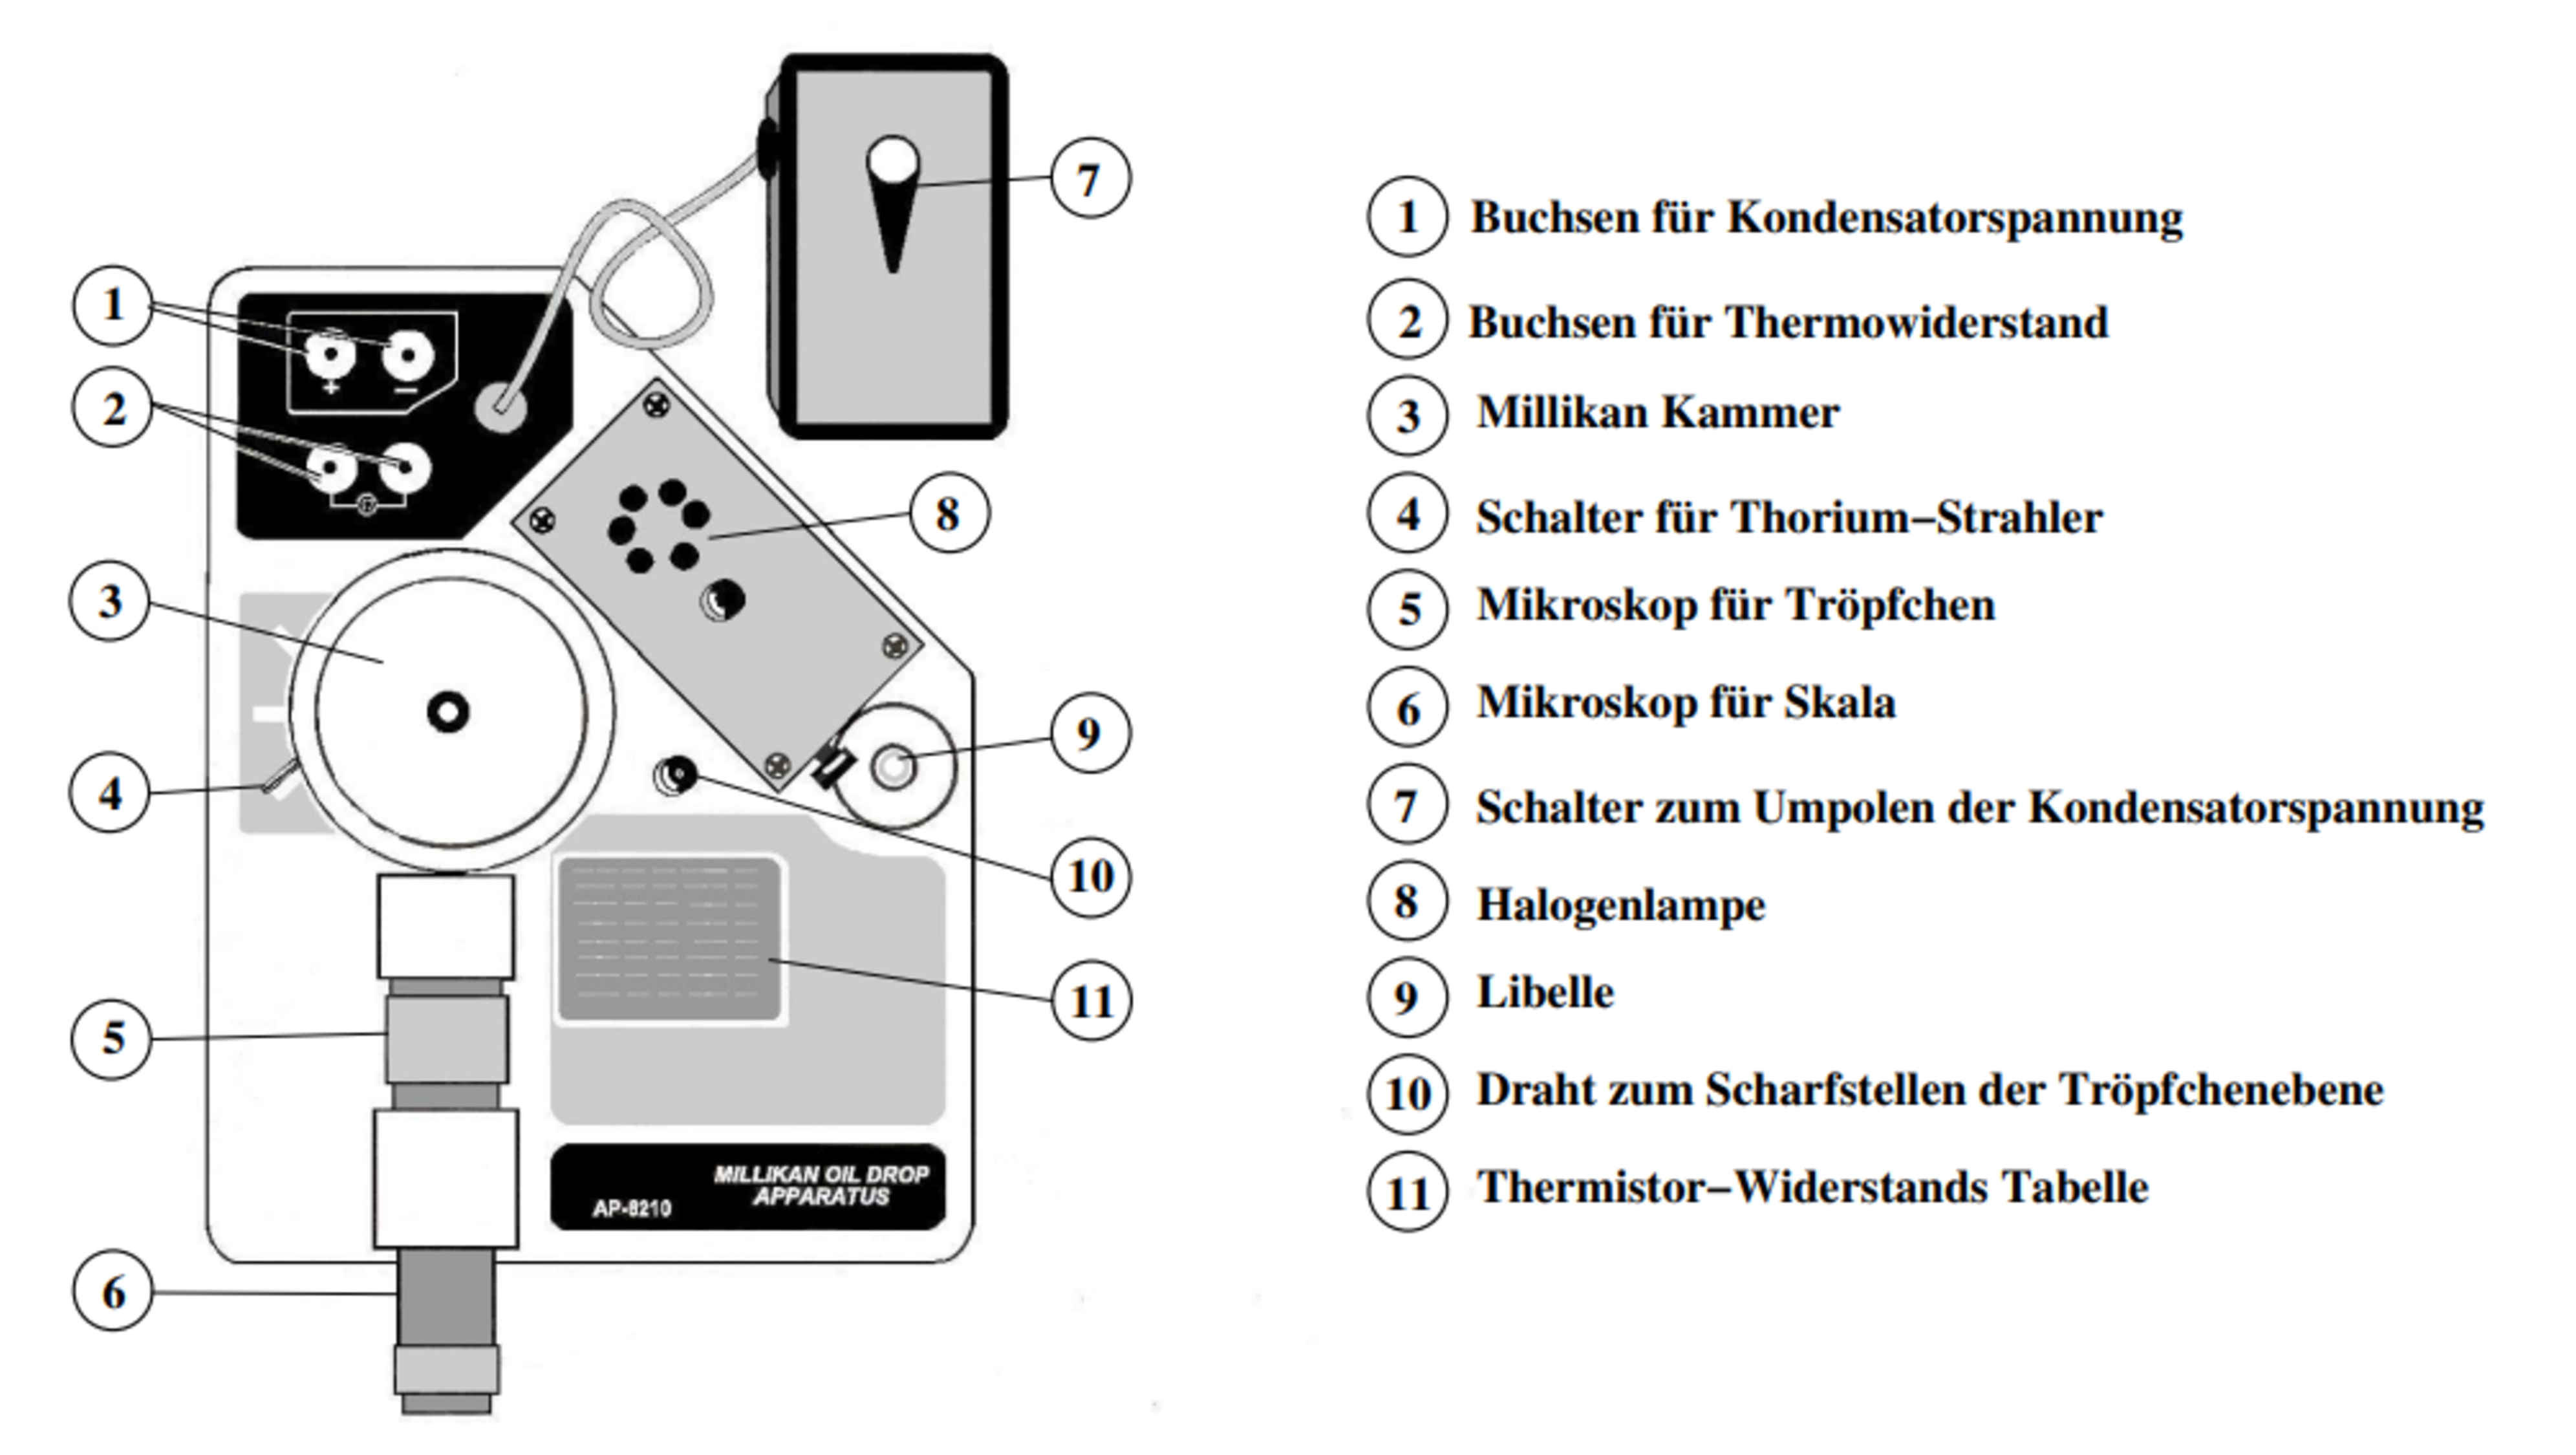
\includegraphics[height = 9cm]{Aufbau.pdf}
    \caption{Aufbau des Millikan-Öltröpfchenversuchs \cite{ap503}.}
    \label{fig:aufbau}
\end{figure}

Dieser besteht aus einer Kammer, die einen Plattenkondensator enthält. Dessen Platten 
haben einen Abstand von $d = (7.6250 \pm 0.0051) \,\unit{\milli\meter}$. Die obere
Platte hat in der Mitte eine Öffnung, durch die die mittels eines Zerstäubers 
entstandenen Öltröpfchen in den Plattenkondensator gelangen. Die Öltröpfchen, welche 
mit einer Halogenlampe angestrahlt werden, können
dann mit einem Mikroskop beobachtet werden.

Mittels des Thermowiderstands wird während der Messung die Temperatur überprüft, da sich
diese durch die Halogenlampe erhöht. Desweiteren kann die Ladung der 
Öltröpfchen durch ein radioaktives $\alpha$-Präparat verändert werden. Das Präparat 
selbst kann abgeschirmt oder aktiviert werden. 